\documentclass[12pt]{article}

\usepackage{fullpage}
\usepackage{mdframed}
\usepackage{colonequals}
\usepackage{algpseudocode}
\usepackage{algorithm}
\usepackage{tcolorbox}
\usepackage[all]{xy}
\usepackage{proof}
\usepackage{mathtools}
\usepackage{bbm}
\usepackage{amssymb}
\usepackage{amsthm}
\usepackage{amsmath}
\usepackage{amsxtra}
\newcommand{\bb}{\mathbb}


\newtheorem{theorem}{Theorem}[section]
\newtheorem{corollary}{Corollary}[theorem]
\newtheorem{lemma}{Lemma}

\newcommand{\mathcat}[1]{\textup{\textbf{\textsf{#1}}}} % for defined terms

\newenvironment{problem}[1]
{\begin{tcolorbox}\noindent\textbf{Problem #1}.}
{\vskip 6pt \end{tcolorbox}}

\newenvironment{enumalph}
{\begin{enumerate}\renewcommand{\labelenumi}{\textnormal{(\alph{enumi})}}}
{\end{enumerate}}

\newenvironment{enumroman}
{\begin{enumerate}\renewcommand{\labelenumi}{\textnormal{(\roman{enumi})}}}
{\end{enumerate}}

\newcommand{\defi}[1]{\textsf{#1}} % for defined terms

\theoremstyle{remark}
\newtheorem*{solution}{Solution}

\setlength{\hfuzz}{4pt}

\newcommand{\calC}{\mathcal{C}}
\newcommand{\calF}{\mathcal{F}}
\newcommand{\C}{\mathbb C}
\newcommand{\N}{\mathbb N}
\newcommand{\Q}{\mathbb Q}
\newcommand{\R}{\mathbb R}
\newcommand{\Z}{\mathbb Z}
\newcommand{\br}{\mathbf{r}}
\newcommand{\RP}{\mathbb{RP}}
\newcommand{\CP}{\mathbb{CP}}
\newcommand{\nbit}[1]{\{0, 1\}^{#1}}
\newcommand{\bits}{\{0, 1\}^{n}}
\newcommand{\bbni}{\bigbreak \noindent}
\newcommand{\norm}[1]{\left\vert\left\vert#1\right\vert\right\vert}

\let\1\relax
\newcommand{\1}{\mathbf{1}}
\newcommand{\fr}[2]{\left(\frac{#1}{#2}\right)}

\newcommand{\vecz}{\mathbf{z}}
\newcommand{\vecr}{\mathbf{r}}
\DeclareMathOperator{\Cinf}{C^{\infty}}
\DeclareMathOperator{\Id}{Id}

\DeclareMathOperator{\Alt}{Alt}
\DeclareMathOperator{\ann}{ann}
\DeclareMathOperator{\codim}{codim}
\DeclareMathOperator{\End}{End}
\DeclareMathOperator{\Hom}{Hom}
\DeclareMathOperator{\id}{id}
\DeclareMathOperator{\M}{M}
\DeclareMathOperator{\Mat}{Mat}
\DeclareMathOperator{\Ob}{Ob}
\DeclareMathOperator{\opchar}{char}
\DeclareMathOperator{\opspan}{span}
\DeclareMathOperator{\rk}{rk}
\DeclareMathOperator{\sgn}{sgn}
\DeclareMathOperator{\Sym}{Sym}
\DeclareMathOperator{\tr}{tr}
\DeclareMathOperator{\img}{img}
\DeclareMathOperator{\CandE}{CandE}
\DeclareMathOperator{\CandO}{CandO}
\DeclareMathOperator{\argmax}{argmax}
\DeclareMathOperator{\first}{first}
\DeclareMathOperator{\last}{last}
\DeclareMathOperator{\cost}{cost}
\DeclareMathOperator{\dist}{dist}
\DeclareMathOperator{\path}{path}
\DeclareMathOperator{\parent}{parent}
\DeclareMathOperator{\argmin}{argmin}
\DeclareMathOperator{\excess}{excess}
\let\Pr\relax
\DeclareMathOperator{\Pr}{\mathbf{Pr}}
\DeclareMathOperator{\Exp}{\mathbb{E}}
\DeclareMathOperator{\Var}{\mathbf{Var}}
\let\limsup\relax
\DeclareMathOperator{\limsup}{limsup}
%Paired Delims
\DeclarePairedDelimiter\ceil{\lceil}{\rceil}
\DeclarePairedDelimiter\floor{\lfloor}{ \rfloor}


\newcommand{\dagstar}{*}

\newcommand{\tbigwedge}{{\textstyle{\bigwedge}}}
\setlength{\parindent}{0pt}
\setlength{\parskip}{5pt}


\begin{document}

\title{CS 40: Computational Complexity}

\author{Sair Shaikh}
\maketitle

% Collaboration Notice: Talked to Henry Scheible '26 to discuss ideas.



\begin{problem}{1}(2.2.9) Compute the homology of the following $2$-complexes:
\begin{enumerate}
	\item The quotient of $S^2$ by identifying the north and south poles to a point.
	\item $S^1 \times (S^1 \vee S^1)$.
	\item The space obtained from $D^2$ by first deleting the interiors of two disjoint subdisks in the interior of $D^2$ and then identifying all three resulting boundary circles via homeomorphisms preserving clockwise orientations.
\end{enumerate}
\end{problem}
\begin{solution}
    \bbni
    \begin{enumerate}
        \item We build the CW complex as follows: 
        \begin{enumerate}
            \item Start with one $0$-cell, representing the identified north and south poles.
            \item Attach $2$ $1$-cells, $a$ and $b$. Think of these are loops from the north to south and south to north poles, respectively (they are loops as the points are identified).
            \item Attach $2$ $2$-cells, along $ab$.  
        \end{enumerate}
        Then, the CW chain complex is as follows:
        \[ 0 \to \Z^2 \xrightarrow{\partial_2} \Z^2 \xrightarrow{\partial_1} \Z^1 \to 0\]
        Then, we compute the homology groups as follows:
        \begin{enumerate}
            \item For $i = 0$, we have that $\img(\partial_1)$ is trivial as all the generators are loops and thus have trivial boundary. Thus, $H_0(X) \cong \Z$. The space has one connected component, so this is expected.
            \item For $i = 1$, we have that $\img(\partial_2)$ is generated by $a+b$, the boundary of both $2$-cells and $\ker(\partial_1) = \Z^2$ as noted before. Thus, $H_1(X) \cong \Z^2/\Z = \Z$. 
            \item For $i = 2$, we have that $\ker(\partial_2) \cong \Z$ as $\img(\partial_2) \cong \Z$, by rank-nullity. Thus, $H_2(X) = \Z$.
            \item Since this is a $2$-dimensional CW complex, we have that $H_i(X) = 0$ for $i > 2$.
        \end{enumerate}
        Overall, we have that:
        \[ H_i(X) = \begin{cases} 
            \Z & i = 0 \\
            \Z & i = 1 \\
            \Z & i = 2 \\
            0 & i > 2
        \end{cases}\]
        \item This space is two tori glued together along a circle. We can build this space as follows: 
        \begin{enumerate}
            \item Start with one $0$-cell. 
            \item Attach $3$ $1$-cells, $a$, $b$, and $c$ to the $0$-cell. 
            \item Attach $2$ $2$-cells, $e_1$ and $e_2$ where $e_1$ is attached to $aca^{-1}c^{-1}$ and $e_2$ is attached to $bcb^{-1}c^{-1}$.
        \end{enumerate}
        Then, the CW chain complex is as follows:
        \[ 0 \to \Z^2 \xrightarrow{\partial_2} \Z^3 \xrightarrow{\partial_1} \Z^1 \to 0\]
        Then, we compute the homology groups as follows:
        \begin{enumerate}
            \item For $i = 0$, we have that $\img(\partial_1)$ is trivial as all generators are loops, thus have trivial boundary. Thus, $H_0(X) \cong \Z$. The space has one connected component, so this is expected.
            \item For $i = 1$, we have that $\ker(\partial_1) \cong \Z^3$ as noted before. Moreover, the $2$-cells have boundary $a + c -a -c = 0$ and $b+c-b-c = 0$ respectively, thus the map is also the $0$ map (we can says this in terms of all $\deg$ being $0$ if one wishes). Thus, $H_1(X) \cong \Z^3/\{0\} = \Z^3$.
            \item For $i = 2$, we have that $\ker(\partial_2) \cong \Z^2$, as the two $2$-cells have trivial boundary. Thus, $H_2(X) = \Z^2$.
            \item Since this is a $2$-dimensional CW complex, we have that $H_i(X) = 0$ for $i > 2$.
        \end{enumerate}
        Overall, we have that:
        \[ H_i(X) = \begin{cases} 
            \Z & i = 0 \\
            \Z^3 & i = 1 \\
            \Z^2 & i = 2 \\
            0 & i > 2
        \end{cases}\]
        \newpage
        \item Notice that the CW complex structure is as follows: \bbni
        \begin{centering}
            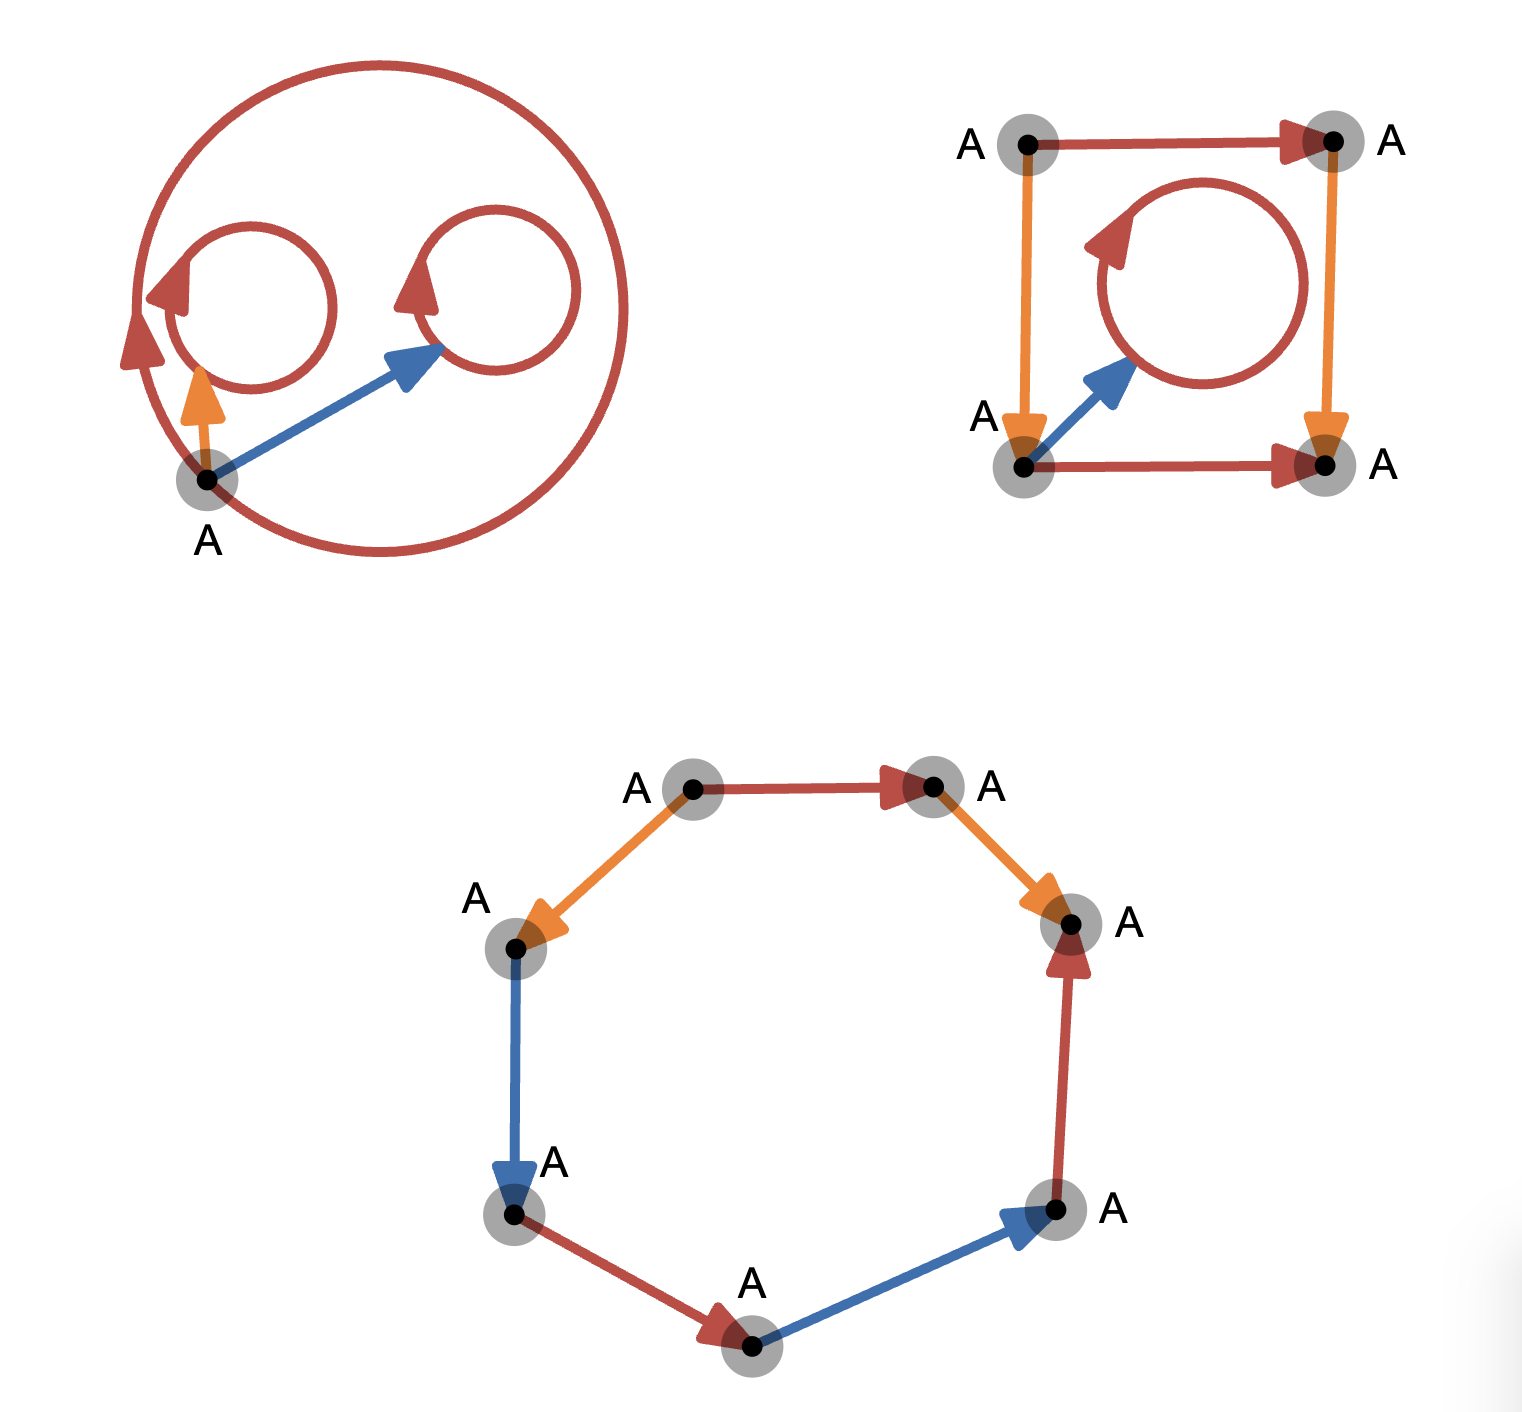
\includegraphics[width=0.8\textwidth]{assets/hwk8_cw.png}
        \end{centering}
    \end{enumerate}
    Thus, $X$ is obtained from taking $1$ $0$-cell, attaching $3$ $1$-cells to get a wedge of $3$ circles, and then attaching a $2$-cell in the manner in the diagram (colors indicated identified edges). Thus, the CW complex looks like: 
    \[ 0 \to \Z \xrightarrow{\partial_2} \Z^3 \xrightarrow{\partial_1} \Z \to 0\]    
    Then, we compute the homology groups as follows:
    \begin{enumerate}
        \item For $i = 0$, note that $\img(\partial_1)$ is trivial as all generators are loops, thus have trivial boundary. Thus, $H_0(X) \cong \Z$. The space has one connected component, so this is expected.
        \item For $i = 1$, we have that $\ker(\partial_1) \cong \Z^2$ as noted before. Moreover, the boundary of the $2$-cell generates $\img(\partial_2)$. Call the red edge $a$, the blue edge $b$, and the orange edge $c$. Then, we have
        \[ \img(\partial_2) = \Z (a +b + a - c - a + c + b) = \Z(a+2b) \cong \Z\]
        Then, noting that $a+2b, b, c$ are linearly independent generators for $(X^1, X_0)$, we note that there are two generators left in the quotient. Thus, $H_1(X) \cong \Z^2$.
        \item For $i = 2$, we have that $\ker(\partial_2)$ is trivial, as the generator maps to a non-zero element. Thus, $H_2(X) = 0$.
        \item For $i > 2$, we have that $H_i(X) = 0$ as this is a $2$-dimensional CW complex.
        Overall, we have that:
        \[ H_i(X) = \begin{cases} 
            \Z & i = 0 \\
            \Z^2 & i = 1 \\
            0 & i \geq 2
            \end{cases}\]
        \end{enumerate} 
\end{solution}

\newpage

\begin{problem}{2}
    Compute the homology of the torus with $n \geq 1$ vertical disks filled in, that is, 
\[ X = (S^1 \times S^1) \bigcup \left( \bigcup_{k=1}^{n} \left\{ e^{2 \pi i k/n}\right\}  \times D^2 \right). \]
\end{problem}

\begin{solution}
    % Since $X$ is path-connected, we know that $H_0(X) \cong \Z$. From Quiz 2, we know that $H_1(X) = \pi_1(X)^{ab} = \Z$. Since $X$ is a $2$ dimensional CW complex, we know that $H_i(X) = 0$ for $i > 2$. Thus, we only need to compute $H_2(X)$. \bbni
    First, to simply, we slide all the disks so that they share a boundary circle homotopically (contract the open cylinders along the torus joining two disks to circles). Then, the CW structures of $X$ is as follows: 
    \begin{enumerate}
        \item $1$ $0$-cell. 
        \item $2$ $1$-cells, call them $a$ and $b$. 
        \item One $2$-cell, call in $e$ attached in the usual way to $aba^{-1}b^{-1}$ and $n$ $2$-cells attached to $b$. 
    \end{enumerate}
    The CW chain complex is then as follows:
    \[ 0 \to \Z^n \oplus \Z \xrightarrow{\partial_2} \Z^2 \xrightarrow{\partial_1} \Z^1 \to 0\]
    Then, we compute the homology groups as follows: 
    \begin{enumerate}
        \item For $i = 0$, note that as every generate of $\Z^n$ is a loop, they have trivial boundary, thus $\partial_1$ is the $0$ map and has trivial image. Thus, $H_0(X) \cong \Z$. We can also see this directly, as $X$ is path-connected.
        \item For $i = 1$, we have that $\ker(\partial_1) \cong \Z^2$, as noted above. Moreover, each of the $n$ disks has $b$ as a boundary, thus $b \in \img(\partial_2)$. Moreover, $\partial_2(e)$ has boundary $a + b - a - b = 0$ (i.e. has deg $0$ for both $a$ and $b$, if we wanna say it that way), thus, $\img(\partial_2) \cong \Z$. Thus, $H_1(X) \cong \Z^2/\Z \cong \Z$. We can also see this directly by abelianizing the fundamental group ($\pi_1(X) = \Z$) from Quiz $2$.
        \item For $i = 2$, we know that $\img(\partial_2) \cong \Z$, as noted above. Thus, $\ker(\partial_2) \cong \Z^n$ by rank-nullity. Thus, we have that $H_2(X) = \ker(\partial_3) \cong \Z^2$.
    \end{enumerate}
    Thus, we have: 
    \[ H_i(X) = \begin{cases}
        \Z & i = 0 \\
        \Z & i = 1 \\
        \Z^n & i = 2 \\
        0 & i > 2
    \end{cases}\]
    
    
    % We look at the CW complex structure. We start with $n+1$ $0$-cells, $e_0^0, \cdots, e_n^0$, and we attach $n+1$ $1$-cells connecting each of them in a loop (i.e. from $e^0_i$ to $e^0_{i+1}$, and $e_n^0$ to $e_0^0$), call them $f_0^1, \cdots, f^1_n$. Then, we attach $n+1$ $1$-cells, one per $e_i^0$, as a loop, call them $e_0^1, \cdots, e_n^1$. Thus, we have a $1$-skeletion consisting of the usual frame of a torus, with $n$ additional vertical circles as $1$-cells. Then, we attach $n+1$ $2$-cells to fill in each empty central region in the frame (i.e. along $e_i^1f_i^1(e_{i+1}^1)^{-1}(f_{i}^1)^{-1}$), call these $f_0^2, \cdots, f_n^2$. Then, finally, attach $n$ disks to each of $e_i^1$ for $i > 0$ to represent the $n$ filled in disks, call these $e_i^2$. This constructs our space $X$. \bbni  
    % In total, we have $n+1$ $0$-cells, $2n+2$ $1$-cells, and $2n+1$ $2$-cells. Thus, we have the following chain complex: 
    % \[ 0 \to \Z^{n+1} \oplus \Z^n \to^{\partial_2} \Z^{n+1} \oplus \Z^{n+1} \to^{\partial_1} \Z^{n+1} \to 0 \]
    % Then, we compute the homology groups as follows: 
    % \begin{enumerate}
    %     \item $H_0(X) = \Z^n/\img(\partial_1)$. However, since our space is path-connected, there is a path between each pair of $0$-cell, thus, all generators of $\Z^n$ differ by a boundary of a path, thus collapse to a single generator. Thus, we have that $H_0(X) \cong \Z$. We could have also just noted that $X$ is path-connected directly to conclude (but I wanted to be more complete).
    %     \item $H_1(X) = \ker(\partial_1)/\img(\partial_2)$. We first calculate $\img(\partial_2)$. We have $2$-cells of the following kind: 
    %     \begin{enumerate}
    %         \item For $e_i^2$ ($i > 0$), the boundary is $e_i^1$. 
    %         \item For $f_i^2$, the boundary is $e_i^1 + f_i^1 - e_{i+1}^1 - f_{i}^1 = e_i^1 - e_{i+1}^2$. These are $0$ for $i \not \in \{0, n\}$. For $i = 0, n$, we get:
    %         \[\]
    % \end{enumerate}
    % Note that $\img(\partial_1) \cong \Z^{n}$ from the previous point. Thus, $\ker{\partial_1} \cong \Z^{n+2}$ by rank-nullity. Thus, we need to compute $\img(\partial_2)$. Note that for the $2$-cells $e_i^2$, the boundaries are $e_i^1$ for $i > 0$, thus these generators die. For $f_i^2$, the boundaries are $e_i^1 + f_i^1 - e_{i+1}^1 - f_{i}^1$. This is non-zero in two cases, $i = 0$ and $i = n$. In these cases, we get: 
    % \[\partial_2(f_0^2) = e_0^1 = \partial_2(f_0^2) \]



    % \end{enumerate}
    % First, consider $n = 1$. Let $A$ be the filled in disk and $B$ be the torus. Clearly, $X = \text{int}(A) \cup \text{int}(B)$. Moreover, $A \cap B$ is a circle $S^1$. Thus, we can apply the Mayer-Vietoris sequence to get:
    % \[\to H_2(A \cap B) \to H_2(A) \oplus H_2(B) \to H_2(X) \to H_1(A \cap B) \to H_1(A) \oplus H_1(B)\]
    % Note that the generator of $H_1(A \cap B) \cong \Z$ is the fundamental circle $S^1$, whose inclusion in $H_1(A)$ is trivial, as $A$ is contractible, and its inclusion in $H_1(B)$ is one of the generators of $H_1(B)$. Thus, the map $H_1(A \cap B) \to H_1(A) \oplus H_1(B)$ has trivial kernel (is injective). Thus, the map $H_2(X) \to H_1(A\cap B)$ is $0$. Noting that $H_2(A \cap B) = 0$ (its a circle), $H_2(A) = 0$ (a disk), $H_2(B) = \Z$, we get:
    % \[ 0 \to \Z \to H_2(X) \to 0 \]
    % Thus, $H_2(X) \cong \Z$. \bbni
    % For $n > 1$, we can use induction.     
\end{solution}

\newpage


\begin{problem}{3}(2.2.21) 
    If a finite CW complex $X$ is a union of subcomplexes $A$ and $B$, show that 
\[ \chi(X) = \chi(A) + \chi(B) - \chi(A \cap B). \]
\end{problem}
\begin{solution}
    Recall the definition of the Euler characteristic:
    \[ \chi(X) = \sum_n (-1)^n |I_n| \]
    where $I_n$ is the set of $n$-cells of $X$. Since $A$ and $B$ are subcomplexes, any cell that intersects with $A$ or $B$ must lie fully within $A$ or $B$, respectively. Since $X = A \cup B$, each cell of $X$ either lies just in $A$ (i.e. in $X\setminus B$), just in $B$ (i.e. in $X\setminus A$), or in both $A$ and $B$ (i.e. in $A \cap B$). For $n$-cells, call these respective sets $I_{n, A}$, $I_{n, B}$, and $I_{n, A \cap B}$. Clearly, by the inclusion-exclusion principle, we have: 
    \[ |I_n| = |I_{n, A}| + |I_{n, B}| - |I_{n, A\cap B}|\]
    Thus, we can write the Euler characteristic of $X$ as:
    \begin{align*}
    \chi(X) &= \sum_n (-1)^n |I_n| \\
    &= \sum_n (-1)^n \left( |I_{n, A}| + |I_{n, B}| - |I_{n, A\cap B}| \right) \\
    &= \sum_n (-1)^n |I_{n, A}| + \sum_n (-1)^n |I_{n, B}| - \sum_n (-1)^n |I_{n, A\cap B}| \\
    &= \chi(A) + \chi(B) - \chi(A \cap B).
    \end{align*}
    Thus, 
    \[ \chi(X) = \chi(A) + \chi(B) - \chi(A \cap B). \]
    % A second proof can be given using the Mayer-Vietoris sequence. Since $A$ and $B$ are subcomplexes of $X$, we have that $X = \text{int}(A) \cup \text{int}(B)$. Thus, we can apply the Mayer-Vietoris sequence to get: 
    % \[ \cdots \to H_i(A \cap B) \to H_i(A) \oplus H_i(B) \to H_i(X) \to H_{i-1}(A \cap B) \to \cdots \]
\end{solution}
\newpage


\begin{problem}{4}(2.2.22) 
    If $X$ is a finite CW complex and $p \colon \widetilde{X} \to X$ is a degree $n$ covering, show that $\chi(\widetilde{X}) = n \cdot \chi(X)$. 
\end{problem}
\begin{solution}
    Let $X$ be $m$-dimensional. It suffices to show that $|I_j(\widetilde{X})| = n |I_j(X)|$ for each $j \leq m$, as: 
    \begin{align*}
    \chi(\widetilde{X}) &= \sum_{k=0}^m (-1)^k |I_k(\widetilde{X})| \\
    &= \sum_{k=0}^m (-1)^k n \cdot |I_k(X)| \\
    &= n \sum_{k=0}^m (-1)^k |I_k(X)| \\
    &= n \cdot \chi(X)
    \end{align*}
    To show this, we claim that $\rho^{-1}(X^{k})$ is a $k$-dimensional CW complex in $\widetilde{X}$ for each $k \geq 0$, with $|I_j(\widetilde X)| = n \cdot |I_j(X)|$ for all $j \leq k$. We proceed by induction. \bbni
    For $k = 0$, we know that for every $0$-cell $x \in X$, there are $n$ distinct preimages under $\rho$ in $\widetilde{X}$, as $p$ is a covering map of degree $n$. Thus, $\widetilde{X}^0 = \rho^{-1}(X^0)$ is a $0$-dimensional CW complex with $|I_0(\widetilde{X})| = n |I_0(X)|$. \bbni
    For $k > 0$, let $e^k$ be a $k$-cell of $X$ with map $\phi: D^k \to X$. Since $\pi_1(D^k, d_0)$ is trivial (for $d_0 \in \text{int}(D^k)$), we have that $\phi_{*}(\pi_1(D^n, d_0))$ is also trivial. Thus, as $D^n$ is path-connected and locally path-connected we can use the universal lifting property to get a unique lift for each pre-image under $\rho$ of $\phi(d_0)$, call these $\phi_1, \ldots, \phi_n: D^k \to \widetilde{X}$. We claim that $\text{int}(\img(\phi_i))$ are disjoint $k$-cells of $\widetilde{X}$ that map homeomorphically to $e^k$ under $p$. \bbni
    For $1 \leq i \leq n$, note that we have: 
    \[ \rho \circ \phi_i = \phi\]
    Then note the following:
    \begin{enumerate}
        \item As $\phi|_{\text{int}(D^k)}$ is a homeomorphism onto $e^k$, so is $\rho \circ \phi_i|_{\text{int}(D^k)}$. Thus, $\rho|_{\phi_i(\text{int}(D^k))}$ is a homeomorphism onto $e^k$, i.e. $\phi_i(\text{int}(D^k)) \cong e^k$. Thus, we have $\phi_i(\text{int}(D^k)) \cong e^k \cong \text{int}(D^k)$.
        \item Note $\rho \circ \phi_i(\delta D^n) = \phi(\delta D^n) \subseteq X^{k-1}$. Then, by the induction hypothesis, we have that $\rho^{-1}(X^{k-1}) = \widetilde{X}^{k-1}$. Thus, $\phi_i(\delta D^n) \subseteq \widetilde{X}^{k-1}$. 
    \end{enumerate}
    Thus, $\phi_i(\text{int}(D^k))$ are $k$-cells of $\widetilde{X}$ for each $i$. Finally, as these cells contain a distinct pre-image of the $\phi(d_0)$, they must be disjoint by uniqueness of the lift. Thus, we have that: 
    \[ \rho^{-1}(e^k) = \bigsqcup_i \phi_i(\text{int}(D^k))\]
    since we have $n$ distinct homeomorphic copies of $e^k$. Thus, considering these as the $k$-cells of $\widetilde{X}$, we have that $\rho^{-1}(X^k) = \widetilde{X}^k$ is a $k$-dimensional CW complex, with $|I_k(\widetilde{X})| = n \cdot |I_k(X)|$. By the induction hypothesis, we have that $|I_j(\widetilde{X})| = n \cdot |I_j(X)|$ for each $j \leq k$. \bbni
    Thus, we note that since $X$ is a finite CW complex of some dimension $m$, so is $\widetilde{X}$ and we have that $|I_j(\widetilde{X})| = n \cdot |I_j(X)|$ for each $j \leq m$. As noted before, this concludes the proof.
\end{solution}
\newpage

\begin{problem}{5}
    Use the previous problem to show that if $\rho \colon \mathbb{RP}^{2n} \to X$ is a covering map where $X$ is a finite CW complex, then $p$ is a homeomorphism.    
\end{problem}
\begin{solution}
    Note that from the previous question, we have that: 
    \[ \chi(\RP^{2n}) = \deg(\rho) \cdot \chi(X)\]
    where $\deg(\rho)$ is the degree of the covering map $\rho$. Moreover, note that we showed: 
    \[ H_i(\RP^{2n}) = \begin{cases}
        \Z & i = 0 \\
        \Z/2\Z & 1 < i < 2n, i \text{ odd } \\
        0 & \text{otherwise}
    \end{cases}\]
    Thus, we can calculate $\chi(\RP^{2n})$ as follows:
    \begin{align*}
        \chi(\RP^{2n}) &= \sum_{i=0}^{2n} (-1)^i \rk(H_i(\RP^{2n})) = 1 
    \end{align*}
    as the free rank of $\Z/2\Z$ is $0$. Thus, we have that: 
    \[\deg(\rho) \cdot \chi(X) = 1\]
    Since both $\deg(\rho)$ and $\chi(X)$ are integers, we have $\deg(\rho) = \chi(X) = \pm 1$. However, as the degree of a covering map cannot be negative, we have that $\deg(\rho) = \chi(X) = 1$. In particular, this means that $\rho$ is a homeomorphism. 
\end{solution}

\end{document}